\documentclass[a4paper, 12pt]{article}

\author{
    b13701220,
    b13703048,
    b13705036,
    b13303079
}
\title{\textbf{Operations Research\\Midterm Project}}
\date{May 2026}

\usepackage[margin=2.3cm]{geometry}
\usepackage{amsmath}
\usepackage{amssymb}
\usepackage{amsthm}
\usepackage{enumitem}
\usepackage{graphicx}
\usepackage{listings, lstautogobble}
\usepackage{booktabs}
\usepackage{float}

\usepackage{tabularray}
\UseTblrLibrary{amsmath, siunitx}

\usepackage{tikz}

\graphicspath{{顧懷允/}{./}}

\setlist{nosep}

\begin{document}
    \maketitle






    \section{Problem 1: Solution to Instance 5}

    Solving the formulated MILP on \texttt{instance05.txt} with Gurobi (Python~3.12, default settings) yields the provably optimal profit \textbf{NT\$\,106{,}800} in well under one second. Below we present the plan in operational language.

    \subsection{Headline}

    \begin{center}
    \begin{tblr}{
    colspec = {X[l] r},
    rowsep = 1pt,
    row{1} = {font=\bfseries},
    }
    Item & Amount (NT\$) \\
    \hline
    Sales revenue from the 8 accepted orders & 117{,}000 \\
    Compensation paid to the 2 rejected customers ($2\times$ revenue) & 10{,}200 \\
    \textbf{Net profit} & \textbf{106{,}800} \\
    \end{tblr}
    \end{center}

    \noindent We accept 8 of 10 orders, decline 2, perform 1 free upgrade, and use 1{,}080 of the 1{,}200 budgeted relocation minutes (90\%). No feasible alternative plan does strictly better.

    \subsection{Order-by-order decision}

    \begin{center}\small
    \begin{tblr}{
    colspec = {c c l l r l c c},
    rowsep = 1pt,
    colsep = 4pt,
    row{1} = {font=\bfseries},
    }
    Order & Lv & Pickup & Return & Rev. & Decision & Car & Upg.\\
    \hline
    1  & 1 & St.1, Day4 01:00 & St.6, Day4 20:00 &  1{,}900 & Reject ($-3{,}800$) & --- & --- \\
    2  & 1 & St.4, Day1 16:00 & St.5, Day3 00:00 &  3{,}200 & Reject ($-6{,}400$) & --- & --- \\
    3  & 1 & St.5, Day2 03:30 & St.1, Day4 11:30 &  5{,}600 & Accept & 3 & No \\
    4  & 1 & St.1, Day3 12:00 & St.2, Day5 15:00 &  5{,}100 & Accept & 1 & No \\
    5  & 2 & St.6, Day1 00:00 & St.6, Day4 20:00 & 36{,}800 & Accept & 6 & No \\
    6  & 1 & St.3, Day4 23:00 & St.4, Day5 14:00 &  1{,}500 & Accept & 4 & \textbf{Yes} \\
    7  & 2 & St.2, Day2 03:30 & St.1, Day4 23:30 & 27{,}200 & Accept & 5 & No \\
    8  & 2 & St.6, Day5 04:30 & St.6, Day5 14:30 &  4{,}000 & Accept & 6 & No \\
    9  & 2 & St.3, Day1 19:30 & St.4, Day4 15:30 & 27{,}200 & Accept & 4 & No \\
    10 & 1 & St.4, Day1 06:00 & St.2, Day5 06:00 &  9{,}600 & Accept & 2 & No \\
    \end{tblr}
    \end{center}

    \noindent\emph{Why decline?} Orders 1 and 2 are small-revenue level-1 jobs whose pickup windows collide with strictly more lucrative commitments: serving them would force the cancellation of orders 4/10 or 7/9 (which together earn over NT\$\,69{,}000). Paying NT\$\,10{,}200 in compensation is cheaper than that opportunity cost. \emph{Free upgrade.} Order 6 (level-1) is most profitably satisfied by the level-2 Car 4, which has just completed Order 9 and sits at a convenient station.

    \subsection{Relocation work orders}

    Five employee-driven moves, totalling 1{,}080 of the 1{,}200 budgeted minutes:

    \begin{center}
    \begin{tblr}{
    colspec = {c c c c l l r},
    rowsep = 1pt,
    row{1} = {font=\bfseries},
    }
    \# & Car & From & To & Depart & Arrive & Duration \\
    \hline
    1 & 2 & St.2 & St.4 & Day1 01:30 & Day1 05:30 & 240 \\
    2 & 4 & St.5 & St.3 & Day1 15:30 & Day1 19:00 & 210 \\
    3 & 5 & St.4 & St.2 & Day1 23:00 & Day2 03:00 & 240 \\
    4 & 3 & St.3 & St.5 & Day1 23:30 & Day2 03:00 & 210 \\
    5 & 4 & St.4 & St.3 & Day4 19:30 & Day4 22:30 & 180 \\
    \hline
    &   &      &      &            & Total      & \textbf{1{,}080} / 1{,}200 \\
    \end{tblr}
    \end{center}

    \subsection{Per-car schedules}

    \begin{itemize}
    \item \textbf{Car 1} (L1, st.1): Order 4 only [pick St.1 Day3 12:00 $\to$ ret St.2 Day5 15:00]. No relocation.
    \item \textbf{Car 2} (L1, st.2): Relocate St.2$\to$St.4 (Day1 01:30, 240 min) $\Rightarrow$ Order 10 [Day1 06:00 $\to$ Day5 06:00 St.2].
    \item \textbf{Car 3} (L1, st.3): Relocate St.3$\to$St.5 (Day1 23:30, 210 min) $\Rightarrow$ Order 3 [Day2 03:30 $\to$ Day4 11:30 St.1].
    \item \textbf{Car 4} (L2, st.5): Relocate St.5$\to$St.3 $\Rightarrow$ Order 9 [Day1 19:30 $\to$ Day4 15:30 St.4]; ready Day4 19:30, relocate St.4$\to$St.3 $\Rightarrow$ Order 6 \emph{(upgrade)} [Day4 23:00 $\to$ Day5 14:00].
    \item \textbf{Car 5} (L2, st.4): Relocate St.4$\to$St.2 $\Rightarrow$ Order 7 [Day2 03:30 $\to$ Day4 23:30 St.1].
    \item \textbf{Car 6} (L2, st.6): Order 5 [Day1 00:00 $\to$ Day4 20:00 St.6]; ready Day5 00:00 $\Rightarrow$ Order 8 [Day5 04:30 $\to$ Day5 14:30 St.6]. No relocation.
    \end{itemize}






    \section{Problem 2, 3: Heuristic Algorithm Design}

    While the devised MILP solves Instance 5 in well under one second, on a larger instance (say $n_K = 10{,}000$) the chain-arc count is $\mathcal{O}(n_C \cdot n_K^2) \approx 10^{11}$, well beyond the three-minute budget. We therefore design a three-tier heuristic that recovers the exact MILP at small scales and degrades gracefully.

    \subsection{Algorithm design}

    To solve the car-rental scheduling problem across varying scales and ensure the program produces a feasible solution within the 3-minute limit, our algorithm adopts a \textbf{Three-Tier Adaptive Architecture}. The key idea is to use different strategies for different instance sizes. Small instances are solved by a Path-flow MIP (the devised model with a tight solver time limit), medium-sized instances by a Revenue-first Insertion Heuristic, and large instances by a fast Heap-Based Chronological Greedy. This achieves a good balance between solution quality and computational efficiency.

    \subsection{Algorithm structure}

    \subsubsection*{Flow chart}
    \begin{figure}[H]
        \centering
        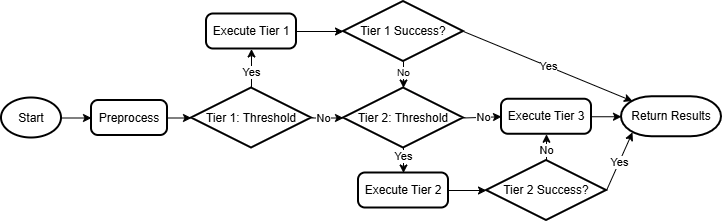
\includegraphics[width=0.88\linewidth]{OR_flowchart.png}
    \end{figure}

    \subsubsection*{Data preprocessing}
    \begin{itemize}
        \item \textbf{Time cache.} Convert all string-formatted times into ``minutes elapsed since 2023/01/01 00:00.'' A dictionary cache avoids repeated string parsing, reducing I/O conversion cost on large instances.
        \item \textbf{Moving-time matrix.} Build a 2-D array \texttt{moving\_time[i][j]} so all relocation-time queries are $\mathcal{O}(1)$.
    \end{itemize}

    \subsubsection*{Tier 1: Small instances (Path-flow MIP)}
    \begin{itemize}
        \item \textbf{Trigger:} $n_K \le 160$ and $n_C\cdot n_K^2 \le 700{,}000$.
        \item \textbf{Logic:} Build the path-flow MILP. Decision variables $x_{c,i,j}$ encode whether car $c$, after serving order $i$, has enough cleaning and moving time to next serve $j$. Gurobi's time limit is set to 20 s; if solved successfully, return the optimal schedule directly.
    \end{itemize}

    \subsubsection*{Tier 2: Medium instances (Revenue-first Insertion Heuristic)}
    \begin{itemize}
        \item \textbf{Trigger:} $n_K \le 6{,}000$ and $n_C\cdot n_K \le 600{,}000$.
        \item \textbf{Logic:} Driven by the intuition of ``maximize business profit.''
        \begin{enumerate}[label=\textbf{\alph*.}]
            \item Sort all orders in descending order of $R_k$.
            \item Process high-revenue orders first; search candidate cars satisfying the level rule (same level or free upgrade).
            \item Use binary search to attempt inserting the new order into the car's existing schedule (sorted by pickup time).
            \item Check the immediately previous and next orders at the insertion position to ensure no conflict after accounting for cleaning and moving times. Assign the car that consumes the least additional relocation budget.
        \end{enumerate}
    \end{itemize}

    \subsubsection*{Tier 3: Large instances (Heap-Based Chronological Greedy)}
    \begin{itemize}
        \item \textbf{Trigger:} ultimate fallback when Tiers 1--2 time out or the instance is too large.
        \item \textbf{Logic:} simulate the passage of time in the real world.
        \begin{enumerate}[label=\textbf{\alph*.}]
            \item Maintain a min-heap for each (station, car-level) pair, keyed by ``earliest ready time.''
            \item Sort orders chronologically by pickup time.
            \item For each order in order, attempt to pop the earliest-ready car from the pickup station's heap in $\mathcal{O}(\log n_C)$.
            \item If no local car is available, scan a pre-built ``nearest-stations'' list, evaluate moving time and remaining budget, and relocate a car from a nearby station. After serving, update the ready time and push the car into the return station's heap.
        \end{enumerate}
    \end{itemize}

    \subsection{Time complexity}

    Let $K = n_K, C = n_C, S = n_S, L = n_L$.

    \smallskip
    \noindent\textit{Preprocessing.} Building the moving-time matrix is $\mathcal{O}(S^2)$ and converting all order times is $\mathcal{O}(K)$:
    \[ T_{\text{prep}} = \mathcal{O}(K + C + S^2). \]

    \noindent\textit{Tier 1 MIP.} The main arc-creation loop is $\mathcal{O}(n_C\cdot n_K^2)$:
    \[ T_{\text{MIP}} = \mathcal{O}(n_C\cdot n_K^2). \]

    \noindent\textit{Tier 2 Insertion heuristic.}
    \begin{itemize}
        \item Sort orders: $\mathcal{O}(n_K\log n_K)$.
        \item For each order, scan all candidate cars and binary-search the insertion position: $\mathcal{O}(n_C\log n_K)$.
        \item Actual insert: $\mathcal{O}(n_K)$ per insertion.
        \item Total: $T_{\text{insertion}} = \mathcal{O}(n_K\cdot n_C\cdot \log n_K + n_K^2)$.
    \end{itemize}

    \smallskip
    \noindent\textit{Tier 3 Heap greedy.}
    \begin{itemize}
        \item Precompute nearest-neighbour list: $\mathcal{O}(n_S^2\log n_S)$.
        \item Sort orders: $\mathcal{O}(n_K\log n_K)$.
        \item Process each order: local-station check $\mathcal{O}(n_L)$, cross-station scan $\mathcal{O}(\text{scan\_limit}\cdot n_L\cdot \log n_C)$.
        \item Total (large $n_S$): $T_{\text{greedy}} = \mathcal{O}(n_S^2\log n_S + n_K\cdot \sqrt{n_S}\cdot n_L\cdot \log n_C)$.
    \end{itemize}






    \section{Problem 4: Heuristic Algorithm Testing}

\end{document}